\documentclass[aspectratio=169, 14pt]{beamer}
\usepackage[utf8]{inputenc}
\usepackage[english]{babel}
\usepackage{tipa}
\usepackage{graphicx}
\usepackage{transparent}
\usepackage[ruled, lined, linesnumbered, commentsnumbered]{algorithm2e}
\newcommand\mycommfont[1]{\small\ttfamily\textcolor{blue}{#1}}
\SetCommentSty{mycommfont}
\renewcommand{\thealgocf}{}
\usepackage{setspace}
\usepackage{pgfplots}
\usepackage{tikz}
\usetikzlibrary{matrix,backgrounds}
\usetikzlibrary{arrows}
\usetikzlibrary {arrows.meta}
\usetikzlibrary{calc,shadows.blur,fit,positioning}
\usetikzlibrary{shapes.multipart,chains}
\usepackage{minted}
\usepackage{fontawesome5}
\usepackage{booktabs}
\usepackage{caption}
\usepackage{hyperref}
\hypersetup{
    colorlinks=true,
    linkcolor=blue,
    filecolor=magenta,      
    urlcolor=cyan,
    }
\urlstyle{same}
\usetheme{metropolis}
\metroset{block=fill}
\usecolortheme{default}
\definecolor{darkmidnightblue}{rgb}{0.0, 0.2, 0.4}
\definecolor{LightGray}{gray}{0.9}

\usepackage[many]{tcolorbox}
\usepackage{varwidth}
\usepackage{environ}
\usepackage{xparse}

\newlength{\bubblesep}
\newlength{\bubblewidth}
\setlength{\bubblesep}{2pt}
\AtBeginDocument{\setlength{\bubblewidth}{.75\textwidth}}
\definecolor{bubblegreen}{RGB}{103,184,104}
\definecolor{bubblegray}{RGB}{241,240,240}

\newcommand{\bubble}[4]{%
  \tcbox[
    on line,
    arc=4.5mm,
    colback=#1,
    colframe=#1,
    #2,
  ]{\color{#3}\begin{varwidth}{\bubblewidth}#4\end{varwidth}}%
}

\ExplSyntaxOn
\seq_new:N \l__ooker_bubbles_seq
\tl_new:N \l__ooker_bubbles_first_tl
\tl_new:N \l__ooker_bubbles_last_tl

\NewEnviron{rightbubbles}
 {
  \begin{flushright}
  \sffamily
  \seq_set_split:NnV \l__ooker_bubbles_seq { \par } \BODY
  \int_compare:nTF { \seq_count:N \l__ooker_bubbles_seq < 2 }
   {
    \bubble{bubblegreen}{rounded~corners}{white}{\BODY}\par
   }
   {
    \seq_pop_left:NN \l__ooker_bubbles_seq \l__ooker_bubbles_first_tl
    \seq_pop_right:NN \l__ooker_bubbles_seq \l__ooker_bubbles_last_tl
    \bubble{bubblegreen}{sharp~corners=southeast}{white}{\l__ooker_bubbles_first_tl}
    \par\nointerlineskip
    \addvspace{\bubblesep}
    \seq_map_inline:Nn \l__ooker_bubbles_seq
     {
      \bubble{bubblegreen}{sharp~corners=east}{white}{##1}
      \par\nointerlineskip
      \addvspace{\bubblesep}
     }
    \bubble{bubblegreen}{sharp~corners=northeast}{white}{\l__ooker_bubbles_last_tl}
    \par
   }
   \end{flushright}
 }
\NewEnviron{leftbubbles}
 {
  \begin{flushleft}
  \sffamily
  \seq_set_split:NnV \l__ooker_bubbles_seq { \par } \BODY
  \int_compare:nTF { \seq_count:N \l__ooker_bubbles_seq < 2 }
   {
    \bubble{bubblegray}{rounded~corners}{black}{\BODY}\par
   }
   {
    \seq_pop_left:NN \l__ooker_bubbles_seq \l__ooker_bubbles_first_tl
    \seq_pop_right:NN \l__ooker_bubbles_seq \l__ooker_bubbles_last_tl
    \bubble{bubblegray}{sharp~corners=southwest}{black}{\l__ooker_bubbles_first_tl}
    \par\nointerlineskip
    \addvspace{\bubblesep}
    \seq_map_inline:Nn \l__ooker_bubbles_seq
     {
      \bubble{bubblegray}{sharp~corners=west}{black}{##1}
      \par\nointerlineskip
      \addvspace{\bubblesep}
     }
    \bubble{bubblegray}{sharp~corners=northwest}{black}{\l__ooker_bubbles_last_tl}\par
   }
  \end{flushleft}
 }
\ExplSyntaxOff

%------------------------------------------------------------
%This block of code defines the information to appear in the
%Title page
\title[Data Structures] %optional
{Data Structures}

\subtitle{Doubly Linked Lists}

\author[CHEN Zhongpu] % (optional)
{CHEN Zhongpu}

\institute[] % (optional)
{
  School of Computing and Artificial Intelligence \\
  \href{mailto:zpchen@swufe.edu.cn}{zpchen@swufe.edu.cn}
}

\date[] % (optional)
{SWUFE, Fall 2022}

%End of title page configuration block
%------------------------------------------------------------


%------------------------------------------------------------
%The next block of commands puts the table of contents at the 
%beginning of each section and highlights the current section:

% \AtBeginSection[]
% {
%   \begin{frame}
%     \frametitle{Table of Contents}
%     \tableofcontents[currentsection]
%   \end{frame}
% }
%------------------------------------------------------------


\begin{document}

%The next statement creates the title page.
\frame{\titlepage}

%---------------------------------------------------------
%This block of code is for the table of contents after
%the title page
% \begin{frame}
% \frametitle{Table of Contents}
% \tableofcontents
% \end{frame}
%--------------------------------------------------------

\begin{frame}
    \frametitle{A Few Tips}

    \begin{exampleblock}{Tips}
        \begin{enumerate}
            \item \faIcon{walking} Slow down. The more you understand, the less you have to memorize.
            \item \faIcon{microphone} Talk about it. Out loud.
            \item \faIcon{beer} Drink water. Lots of it.
        \end{enumerate}        
    \end{exampleblock}

\end{frame}

\begin{frame}[fragile]
    \begin{leftbubbles}
Hi, Alice. Can you describe a linked list in plain language? It looks like a chain.        
    \end{leftbubbles}
\begin{rightbubbles}
Sure. That's a great analogy. It contains nodes where each node contains a data field and a link to the next node in the list, and that's why it is linked.  
\end{rightbubbles}

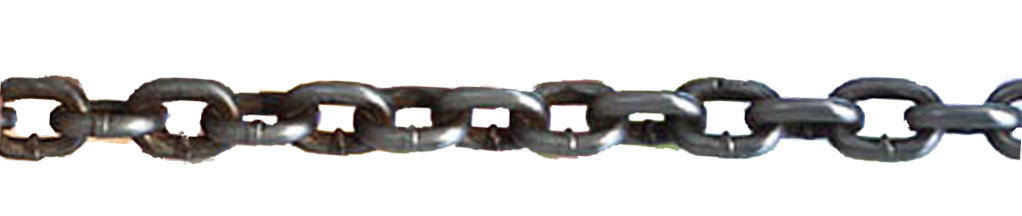
\includegraphics[width=.5\textwidth]{week6/chain}

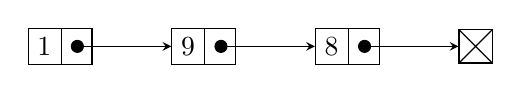
\begin{tikzpicture}[list/.style={rectangle split, rectangle split parts=2,
    draw, rectangle split horizontal}, >=stealth, start chain]

  \node[list,on chain] (A) {1};
  \node[list,on chain] (B) {9};
  \node[list,on chain] (C) {8};
  \node[on chain,draw,inner sep=6pt] (D) {};
  \draw (D.north east) -- (D.south west);
  \draw (D.north west) -- (D.south east);
  \draw[*->] let \p1 = (A.two), \p2 = (A.center) in (\x1,\y2) -- (B);
  \draw[*->] let \p1 = (B.two), \p2 = (B.center) in (\x1,\y2) -- (C);
  \draw[*->] let \p1 = (C.two), \p2 = (C.center) in (\x1,\y2) -- (D);

\end{tikzpicture}

\end{frame}

\begin{frame}[fragile]

\begin{leftbubbles}
Got it. So, as long as I have the \alert{\texttt{head}} node, I am able to scan the elements from left to right, right?
\end{leftbubbles}

\begin{rightbubbles}
Yes, exactly. Do you know how to add a new element into the front of a linked list?
\end{rightbubbles}

\begin{leftbubbles}
Well, it's a bit challenging. Step1: create a new node \alert{x}. Step 2: update \alert{x}'s next to \alert{head}.
\end{leftbubbles}

\begin{rightbubbles}
Close. What else do you need to do?
\end{rightbubbles}

\end{frame}

\begin{frame}

    \begin{leftbubbles}
Oh, a final step: update \alert{head} to \alert{x}! It is a new head after all. But I feel there is still a huge gap to write down the pseudo-code. Let alone the Python or Java code.
    \end{leftbubbles}

\begin{rightbubbles}
Basically, it can be done by a direct ``translation".
\end{rightbubbles}

\begin{table}
    \begin{tabular}{ll}
      \toprule
      Steps & Pseudo-code \\
      \midrule
      Create a new node $x$ & $x \gets Node(element)$ \\
      Update $x$'s next & $x.next \gets head$ \\
      Update $head$ & $head \gets x$\\
      \bottomrule
    \end{tabular}
\end{table}

\end{frame}

\begin{frame}[fragile]
    \begin{leftbubbles}
That's amazing. I think translating it into Python code is similar. Thanks, Alice. I already feel much confident now.
    \end{leftbubbles}
 
\begin{columns}
\column{.5\textwidth}
\scalebox{.85}{  
    \begin{algorithm}[H]
    \caption{addFirst(head, element)}
    $x\gets Node(element)$ \\
    $x.next\gets head$ \\
    $head\gets x$
    \end{algorithm}
}
\column{.5\textwidth} 
\begin{minted}[bgcolor=LightGray, baselinestretch=1]{python}
def add_first(self, item):
    node = Node(item)
    node.next = self._head
    self._head = node
\end{minted}
\end{columns}

\end{frame}

\begin{frame}
\frametitle{A Small Quiz}
{\large \faIcon{question-circle}} What does the following code do?
    \scalebox{.85}{  
        \begin{algorithm}[H]
        \caption{someOperation}
        \If{isEmpty(head)} {
            raise an error
        } \Else {
            $head\gets head.next$
        }
        \end{algorithm}
    } 
\end{frame}

\begin{frame}
    \frametitle{A Small Quiz}
    {\large \faIcon{question-circle}} Please describe the main idea of \texttt{removeLast()}? And what is the time complexity?

    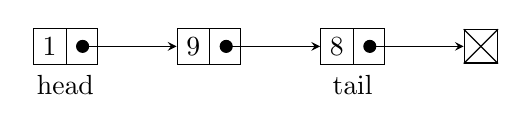
\begin{tikzpicture}[list/.style={rectangle split, rectangle split parts=2,
        draw, rectangle split horizontal}, >=stealth, start chain]
    
      \node[list,on chain] (A) {1};
      \node[list,on chain] (B) {9};
      \node[list,on chain] (C) {8};
      \node[on chain,draw,inner sep=6pt] (D) {};
      \draw (D.north east) -- (D.south west);
      \draw (D.north west) -- (D.south east);
      \draw[*->] let \p1 = (A.two), \p2 = (A.center) in (\x1,\y2) -- (B);
      \draw[*->] let \p1 = (B.two), \p2 = (B.center) in (\x1,\y2) -- (C);
      \draw[*->] let \p1 = (C.two), \p2 = (C.center) in (\x1,\y2) -- (D);
    
      \node[below=of A, yshift=1cm]{\alert{head}};
      \node[below=of C, yshift=1cm]{\alert{tail}};
    
    \end{tikzpicture}

    \pause
    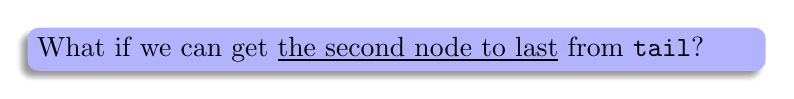
\begin{tikzpicture}
        \node[fill=blue!30,blur shadow={shadow xshift=-0.5ex},
        text width=26em,anchor=south west,rounded corners]
        {What if we can get \underline{the second node to last} from \alert{\texttt{tail}}?};
    \end{tikzpicture}

\end{frame}

{
    % \usebackgroundtemplate{\transparent{0.3}{\begin{picture}
    %     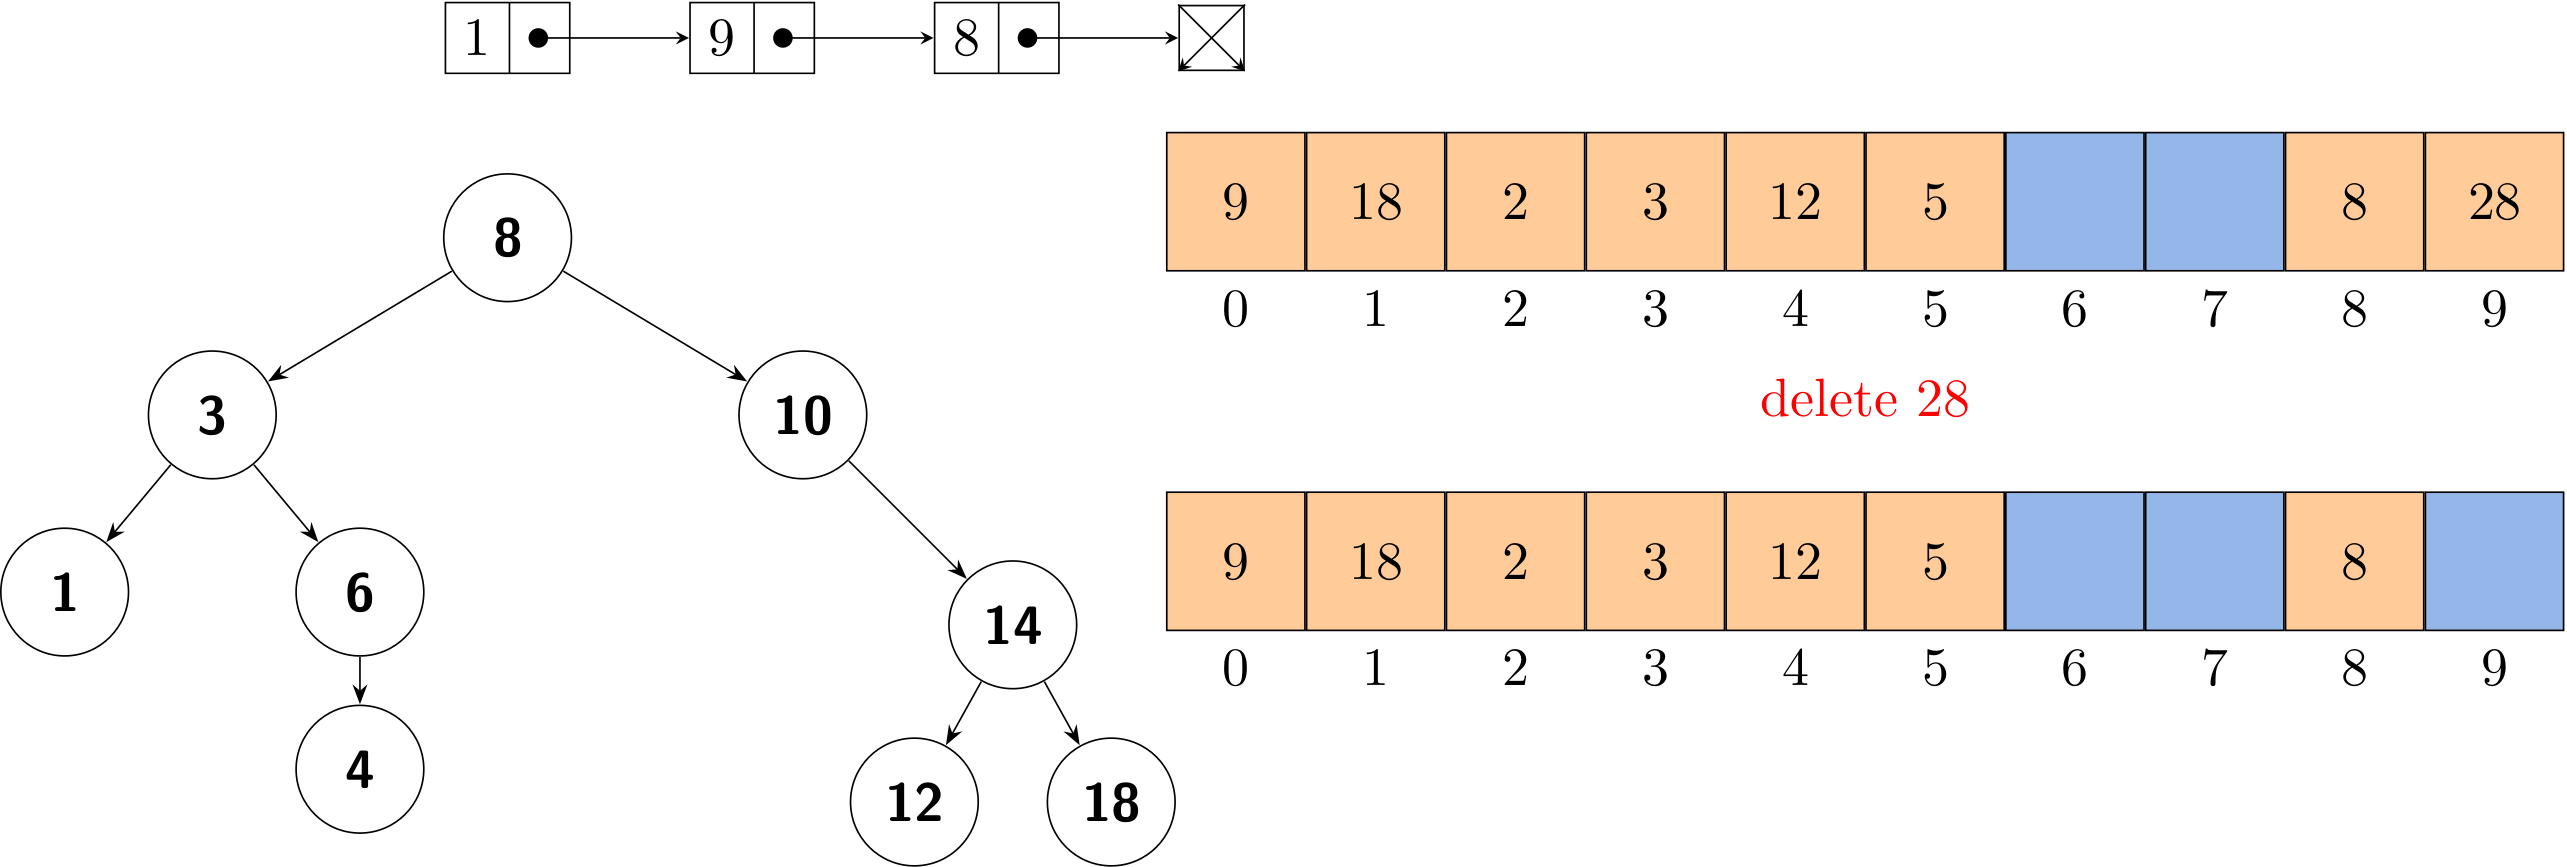
\includegraphics[height=0.7\paperheight]{cover}
    % \end{picture}    
    % }}
\usebackgroundtemplate{
  \tikz[overlay,remember picture] 
  \node[opacity=0.3, at=(current page.south east),anchor=south east, yshift=2cm,xshift=4cm] {
    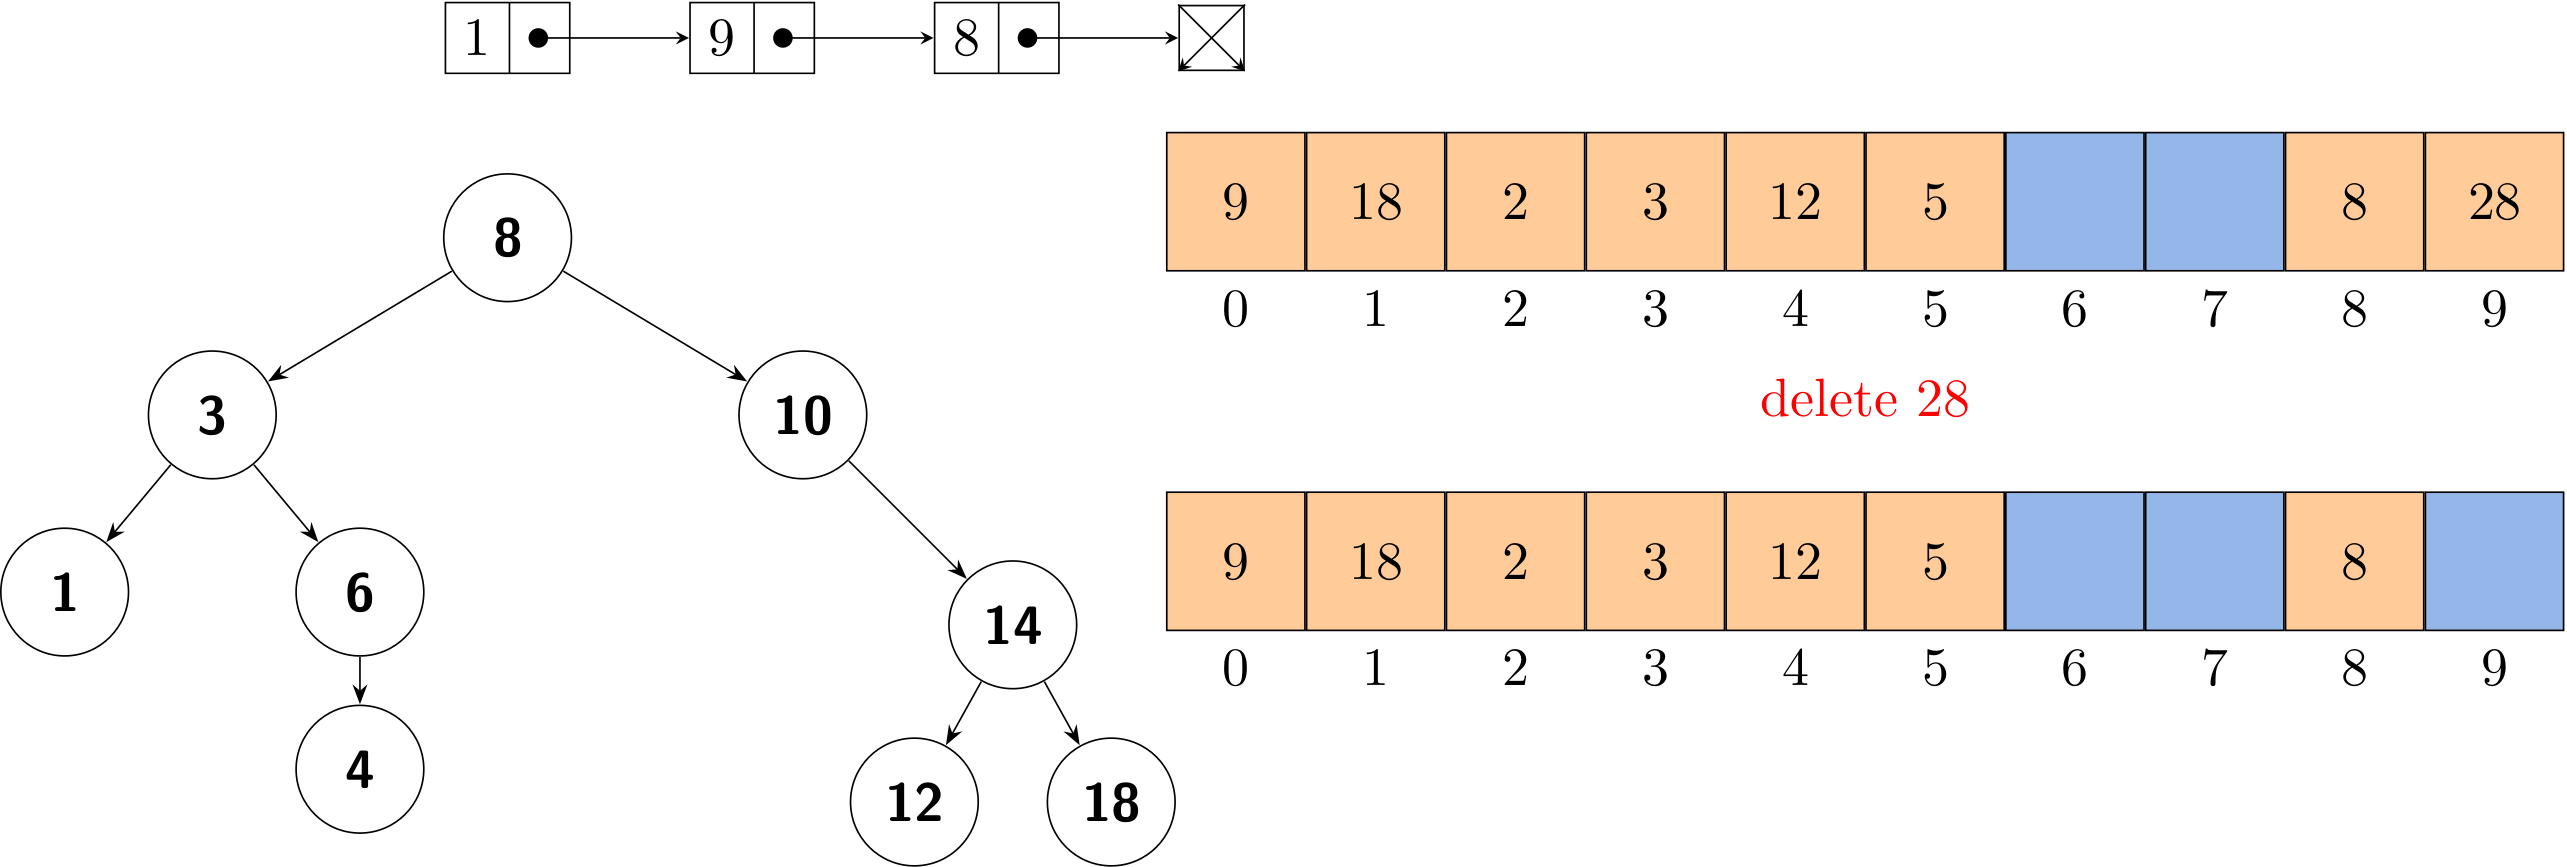
\includegraphics[height=0.6\paperheight]{cover}};
}
    \begin{frame}
        \section{\textcolor{darkmidnightblue}{1. Doubly Linked Lists}}
    \end{frame}

}

\begin{frame}
    \frametitle{1.1 Doubly Linked Lists}

By default, a linked list is a \textbf{singly linked list}, whose node has only one link to the \alert{\texttt{next}} node. If every node also has a link to its \alert{\texttt{previous}} node, it is called \textbf{doubly linked list}.

    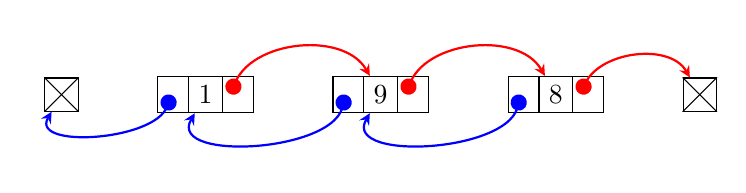
\begin{tikzpicture}[list/.style={rectangle split, rectangle split parts=3,
        draw, rectangle split horizontal}, >=stealth, start chain]


        \node[on chain,draw,inner sep=6pt] (AA) {};
        \draw (AA.north east) -- (AA.south west);
        \draw (AA.north west) -- (AA.south east);
      \node[list,on chain] (A) {\nodepart{second}1};
      \node[list,on chain] (B) {\nodepart{second}9};
      \node[list,on chain] (C) {\nodepart{second}8};
      \node[on chain,draw,inner sep=6pt] (D) {};
      \draw (D.north east) -- (D.south west);
      \draw (D.north west) -- (D.south east);



      \draw[*->, red, thick] let \p1 = (A.three), \p2 = (A.center) in (\x1,\y2) to[out=80,in=120] (B);
      \draw[*->, blue, thick] let \p1 = (A.one), \p2 = (A.center) in (\x1,\y2) to[out=-80,in=-120] (AA);

      \draw[*->, red, thick] let \p1 = (B.three), \p2 = (B.center) in (\x1,\y2) to[out=80,in=120] (C);
      \draw[*->, blue, thick] let \p1 = (B.one), \p2 = (B.center) in (\x1,\y2) to[out=-80,in=-120] (A);

      \draw[*->, red, thick] let \p1 = (C.three), \p2 = (C.center) in (\x1,\y2) to[out=80,in=120] (D);
      \draw[*->, blue, thick] let \p1 = (C.one), \p2 = (C.center) in (\x1,\y2) to[out=-80,in=-120] (B);
    
    \end{tikzpicture}

\end{frame}

\begin{frame}[fragile]
The node in a doubly linked list contains: \alert{\texttt{item}}, \alert{\texttt{prev}} and \alert{\texttt{next}}.

\begin{minted}[bgcolor=LightGray]{python}
class Node:
    def __init__(self, item=None, prev=None, nxt=None):
        self.item = item
        self.prev = prev
        self.next = nxt 
\end{minted}

\end{frame}

\begin{frame}[fragile]
    \frametitle{Exercise}
{\large \faIcon{code}} Given a doubly linked list with \alert{\texttt{head}} and \alert{\texttt{tail}}, how to remove the last node?

\begin{itemize}
    \item \textbf{Case 1}: the list is empty.
    \item \textbf{Case 2}: the size is 1.
    \item \textbf{Case 3}: the size is greater than 1.
\end{itemize}

    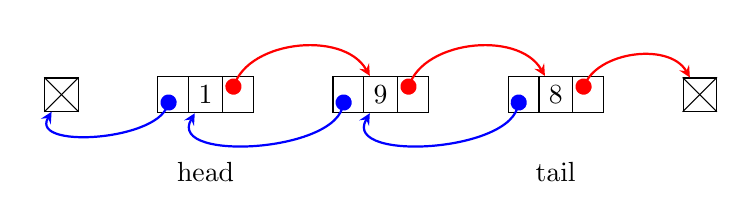
\begin{tikzpicture}[list/.style={rectangle split, rectangle split parts=3,
        draw, rectangle split horizontal}, >=stealth, start chain]


        \node[on chain,draw,inner sep=6pt] (AA) {};
        \draw (AA.north east) -- (AA.south west);
        \draw (AA.north west) -- (AA.south east);
      \node[list,on chain] (A) {\nodepart{second}1};
      \node[list,on chain] (B) {\nodepart{second}9};
      \node[list,on chain] (C) {\nodepart{second}8};
      \node[on chain,draw,inner sep=6pt] (D) {};
      \draw (D.north east) -- (D.south west);
      \draw (D.north west) -- (D.south east);



      \draw[*->, red, thick] let \p1 = (A.three), \p2 = (A.center) in (\x1,\y2) to[out=80,in=120] (B);
      \draw[*->, blue, thick] let \p1 = (A.one), \p2 = (A.center) in (\x1,\y2) to[out=-80,in=-120] (AA);

      \draw[*->, red, thick] let \p1 = (B.three), \p2 = (B.center) in (\x1,\y2) to[out=80,in=120] (C);
      \draw[*->, blue, thick] let \p1 = (B.one), \p2 = (B.center) in (\x1,\y2) to[out=-80,in=-120] (A);

      \draw[*->, red, thick] let \p1 = (C.three), \p2 = (C.center) in (\x1,\y2) to[out=80,in=120] (D);
      \draw[*->, blue, thick] let \p1 = (C.one), \p2 = (C.center) in (\x1,\y2) to[out=-80,in=-120] (B);

      \node[below=of A, yshift=.5cm]{\alert{head}};
      \node[below=of C, yshift=.5cm]{\alert{tail}};
    
    \end{tikzpicture}
    
\end{frame}

\begin{frame}

    \scalebox{.85}{  
        \begin{algorithm}[H]
        \setstretch{1}
        \caption{removeLast(head, tail)}
        \If{isEmpty(head)} {
            \tcp{case 1: it is empty}
            raise an error
        }\ElseIf{head == tail} {
            \tcp{case 2: the size is 1}
            $head\gets null$ \\
            $tail\gets null$ 
        }\Else{
            \tcp{case 3: the size is greater than 1}
            $x\gets tail.prev$\\
            $x.next\gets null$ \\
            $tail\gets x$
        }
        \end{algorithm}
    } 

\end{frame}

\begin{frame}
\frametitle{1.2 Revisit}
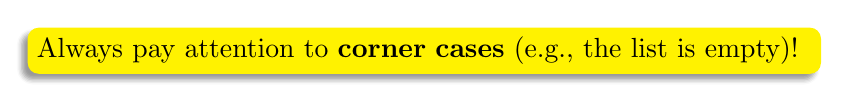
\begin{tikzpicture}
    \node[fill=yellow,blur shadow={shadow xshift=-0.5ex},
    text width=28em,anchor=south west,rounded corners]
    {Always pay attention to \textbf{corner cases} (e.g., the list is empty)!};
\end{tikzpicture}

\begin{exampleblock}{Insight}
The fewer cases, the simpler code.
\end{exampleblock}

\pause

To make it possible, we can introduce \alert{sentinels} (i.e., \emph{dummy nodes}) for linked lists.

    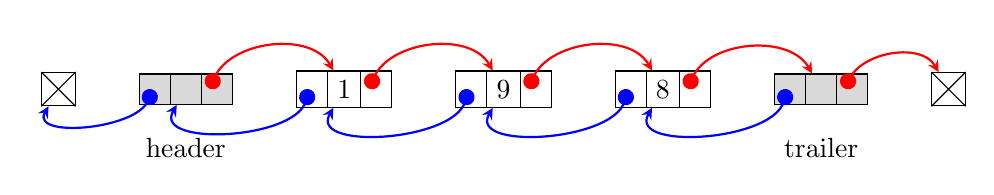
\begin{tikzpicture}[list/.style={rectangle split, rectangle split parts=3,
        draw, rectangle split horizontal}, >=stealth, start chain, node distance=.8cm]

        \node[on chain,draw,inner sep=6pt] (AA) {};
        \draw (AA.north east) -- (AA.south west);
        \draw (AA.north west) -- (AA.south east);

        \node[list, on chain, fill=gray!30] (header) {};
      \node[list,on chain] (A) {\nodepart{second}1};
      \node[list,on chain] (B) {\nodepart{second}9};
      \node[list,on chain] (C) {\nodepart{second}8};
      \node[list, on chain, fill=gray!30] (trailer) {};
      \node[on chain,draw,inner sep=6pt] (D) {};
      \draw (D.north east) -- (D.south west);
      \draw (D.north west) -- (D.south east);


            
      \draw[*->, red, thick] let \p1 = (header.three), \p2 = (header.center) in (\x1,\y2) to[out=80,in=120] (A);
      \draw[*->, red, thick] let \p1 = (A.three), \p2 = (A.center) in (\x1,\y2) to[out=80,in=120] (B);
      \draw[*->, blue, thick] let \p1 = (A.one), \p2 = (A.center) in (\x1,\y2) to[out=-80,in=-120] (header);
      \draw[*->, blue, thick] let \p1 = (header.one), \p2 = (header.center) in (\x1,\y2) to[out=-80,in=-120] (AA);

      \draw[*->, red, thick] let \p1 = (B.three), \p2 = (B.center) in (\x1,\y2) to[out=80,in=120] (C);
      \draw[*->, blue, thick] let \p1 = (B.one), \p2 = (B.center) in (\x1,\y2) to[out=-80,in=-120] (A);

      \draw[*->, red, thick] let \p1 = (C.three), \p2 = (C.center) in (\x1,\y2) to[out=80,in=120] (trailer);
      \draw[*->, blue, thick] let \p1 = (C.one), \p2 = (C.center) in (\x1,\y2) to[out=-80,in=-120] (B);
     \draw[*->, red, thick] let \p1 = (trailer.three), \p2 = (trailer.center) in (\x1,\y2) to[out=80,in=120] (D);
      \draw[*->, blue, thick] let \p1 = (trailer.one), \p2 = (trailer.center) in (\x1,\y2) to[out=-80,in=-120] (C);

      \node[below=of header, yshift=.5cm]{\alert{header}};
      \node[below=of trailer, yshift=.5cm]{\alert{trailer}};
    
    \end{tikzpicture}

\end{frame}

\begin{frame}
        \scalebox{.85}{  
        \begin{algorithm}[H]
        \setstretch{1}
        \caption{removeLast(header, trailer)}
        \If{isEmpty(head)} {
            \tcp{case 1: it is empty}
            raise an error
        }\Else{
            \tcp{case 2: it is not empty}
            $x\gets trailer.prev$ \\
            $predecessor\gets x.prev$ \\
            $predecessor.next\gets trailer$ \\
            $trailer.prev\gets predecessor$
        }
        \end{algorithm}
    }   
    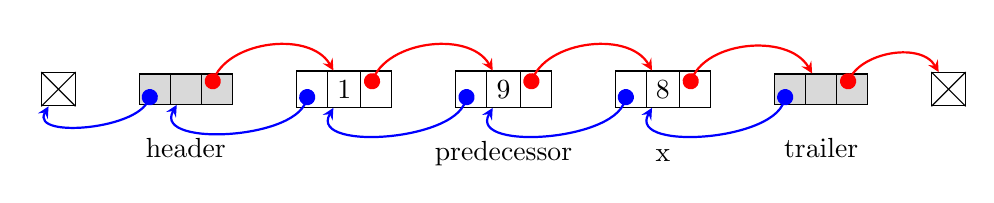
\begin{tikzpicture}[list/.style={rectangle split, rectangle split parts=3,
        draw, rectangle split horizontal}, >=stealth, start chain, node distance=.8cm]

        \node[on chain,draw,inner sep=6pt] (AA) {};
        \draw (AA.north east) -- (AA.south west);
        \draw (AA.north west) -- (AA.south east);

        \node[list, on chain, fill=gray!30] (header) {};
      \node[list,on chain] (A) {\nodepart{second}1};
      \node[list,on chain] (B) {\nodepart{second}9};
      \node[list,on chain] (C) {\nodepart{second}8};
      \node[list, on chain, fill=gray!30] (trailer) {};
      \node[on chain,draw,inner sep=6pt] (D) {};
      \draw (D.north east) -- (D.south west);
      \draw (D.north west) -- (D.south east);

      \draw[*->, red, thick] let \p1 = (header.three), \p2 = (header.center) in (\x1,\y2) to[out=80,in=120] (A);
      \draw[*->, red, thick] let \p1 = (A.three), \p2 = (A.center) in (\x1,\y2) to[out=80,in=120] (B);
      \draw[*->, blue, thick] let \p1 = (A.one), \p2 = (A.center) in (\x1,\y2) to[out=-80,in=-120] (header);
      \draw[*->, blue, thick] let \p1 = (header.one), \p2 = (header.center) in (\x1,\y2) to[out=-80,in=-120] (AA);

      \draw[*->, red, thick] let \p1 = (B.three), \p2 = (B.center) in (\x1,\y2) to[out=80,in=120] (C);
      \draw[*->, blue, thick] let \p1 = (B.one), \p2 = (B.center) in (\x1,\y2) to[out=-80,in=-120] (A);

      \draw[*->, red, thick] let \p1 = (C.three), \p2 = (C.center) in (\x1,\y2) to[out=80,in=120] (trailer);
      \draw[*->, blue, thick] let \p1 = (C.one), \p2 = (C.center) in (\x1,\y2) to[out=-80,in=-120] (B);
     \draw[*->, red, thick] let \p1 = (trailer.three), \p2 = (trailer.center) in (\x1,\y2) to[out=80,in=120] (D);
      \draw[*->, blue, thick] let \p1 = (trailer.one), \p2 = (trailer.center) in (\x1,\y2) to[out=-80,in=-120] (C);

      \node[below=of header, yshift=.5cm]{\alert{header}};
      \node[below=of trailer, yshift=.5cm]{\alert{trailer}};
      \node[below=of C, yshift=.4cm] {\alert{x}};
      \node[below=of B, yshift=.5cm] {\alert{predecessor}};
    \end{tikzpicture}

\end{frame}

\begin{frame}
    \frametitle{Exercise}
   {\large \faIcon{code}} Given a \texttt{node} in a doubly linked list, how to remove it?

       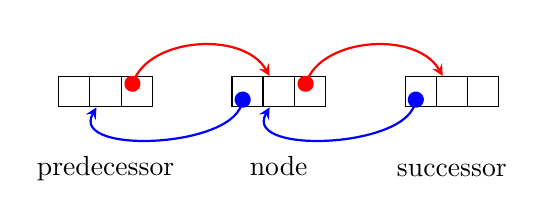
\begin{tikzpicture}[list/.style={rectangle split, rectangle split parts=3,
        draw, rectangle split horizontal}, >=stealth, start chain,]


      \node[list,on chain] (A) {};
      \node[list,on chain] (B) {};
      \node[list,on chain] (C) {};

      \draw[*->, red, thick] let \p1 = (A.three), \p2 = (A.center) in (\x1,\y2) to[out=80,in=120] (B);

      \draw[*->, red, thick] let \p1 = (B.three), \p2 = (B.center) in (\x1,\y2) to[out=80,in=120] (C);
      \draw[*->, blue, thick] let \p1 = (B.one), \p2 = (B.center) in (\x1,\y2) to[out=-80,in=-120] (A);

      \draw[*->, blue, thick] let \p1 = (C.one), \p2 = (C.center) in (\x1,\y2) to[out=-80,in=-120] (B);

      \node[below=of A, yshift=.5cm]{\alert{predecessor}};
      \node[below=of B, yshift=.5cm]{\alert{node}};
      \node[below=of C, yshift=.4cm] {\alert{successor}};
    \end{tikzpicture}

\end{frame}

\begin{frame}
       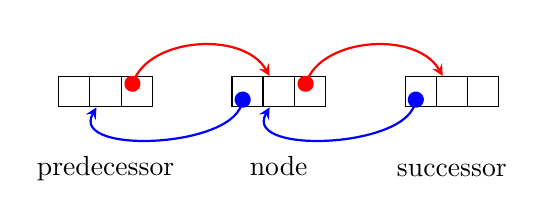
\begin{tikzpicture}[list/.style={rectangle split, rectangle split parts=3,
        draw, rectangle split horizontal}, >=stealth, start chain,]


      \node[list,on chain] (A) {};
      \node[list,on chain] (B) {};
      \node[list,on chain] (C) {};

      \draw[*->, red, thick] let \p1 = (A.three), \p2 = (A.center) in (\x1,\y2) to[out=80,in=120] (B);

      \draw[*->, red, thick] let \p1 = (B.three), \p2 = (B.center) in (\x1,\y2) to[out=80,in=120] (C);
      \draw[*->, blue, thick] let \p1 = (B.one), \p2 = (B.center) in (\x1,\y2) to[out=-80,in=-120] (A);

      \draw[*->, blue, thick] let \p1 = (C.one), \p2 = (C.center) in (\x1,\y2) to[out=-80,in=-120] (B);

      \node[below=of A, yshift=.5cm]{\alert{predecessor}};
      \node[below=of B, yshift=.5cm]{\alert{node}};
      \node[below=of C, yshift=.4cm] {\alert{successor}};
    \end{tikzpicture}

\scalebox{.9}{  
    \begin{algorithm}[H]
        \caption{remove(node)}
        $predecessor\gets node.prev$ \\
        $successor\gets node.next$ \\
        $predecessor.next\gets successor$ \\
        $successor.prev\gets predecessor$
    \end{algorithm}
}
    
\pause
{\large \faIcon{question-circle}} How to implement \texttt{removeLast()} and \texttt{removeFirst()} based on \texttt{remove()}?
\end{frame}

\begin{frame}
    \frametitle{1.3 addFirst()}
    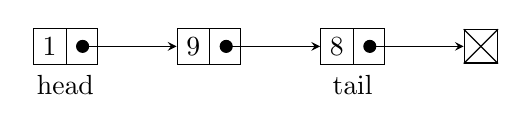
\begin{tikzpicture}[list/.style={rectangle split, rectangle split parts=2,
        draw, rectangle split horizontal}, >=stealth, start chain]
    
      \node[list,on chain] (A) {1};
      \node[list,on chain] (B) {9};
      \node[list,on chain] (C) {8};
      \node[on chain,draw,inner sep=6pt] (D) {};
      \draw (D.north east) -- (D.south west);
      \draw (D.north west) -- (D.south east);
      \draw[*->] let \p1 = (A.two), \p2 = (A.center) in (\x1,\y2) -- (B);
      \draw[*->] let \p1 = (B.two), \p2 = (B.center) in (\x1,\y2) -- (C);
      \draw[*->] let \p1 = (C.two), \p2 = (C.center) in (\x1,\y2) -- (D);

      \node[below=of A, yshift=1cm]{\alert{head}};
      \node[below=of C, yshift=1cm]{\alert{tail}};
    \end{tikzpicture}
    
    \scalebox{.85}{  
        \begin{algorithm}[H]
        \caption{addFirst(head, tail, element)}
        \tcp{singly linked list}
        $head\gets Node(element, head)$ \\
        \If{tail == null} {
            $tail\gets head$
        }
        \end{algorithm}
    } 

\end{frame}

\begin{frame}

        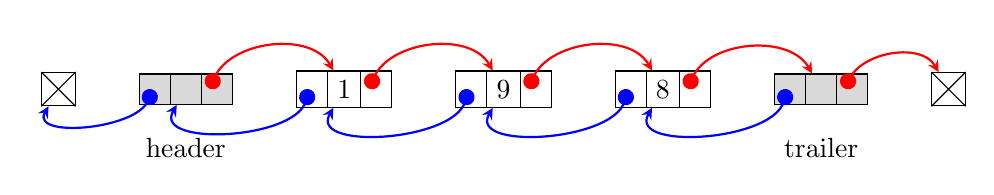
\begin{tikzpicture}[list/.style={rectangle split, rectangle split parts=3,
        draw, rectangle split horizontal}, >=stealth, start chain, node distance=.8cm]

        \node[on chain,draw,inner sep=6pt] (AA) {};
        \draw (AA.north east) -- (AA.south west);
        \draw (AA.north west) -- (AA.south east);

        \node[list, on chain, fill=gray!30] (header) {};
      \node[list,on chain] (A) {\nodepart{second}1};
      \node[list,on chain] (B) {\nodepart{second}9};
      \node[list,on chain] (C) {\nodepart{second}8};
      \node[list, on chain, fill=gray!30] (trailer) {};
      \node[on chain,draw,inner sep=6pt] (D) {};
      \draw (D.north east) -- (D.south west);
      \draw (D.north west) -- (D.south east);

      \draw[*->, red, thick] let \p1 = (header.three), \p2 = (header.center) in (\x1,\y2) to[out=80,in=120] (A);
      \draw[*->, red, thick] let \p1 = (A.three), \p2 = (A.center) in (\x1,\y2) to[out=80,in=120] (B);
      \draw[*->, blue, thick] let \p1 = (A.one), \p2 = (A.center) in (\x1,\y2) to[out=-80,in=-120] (header);
      \draw[*->, blue, thick] let \p1 = (header.one), \p2 = (header.center) in (\x1,\y2) to[out=-80,in=-120] (AA);

      \draw[*->, red, thick] let \p1 = (B.three), \p2 = (B.center) in (\x1,\y2) to[out=80,in=120] (C);
      \draw[*->, blue, thick] let \p1 = (B.one), \p2 = (B.center) in (\x1,\y2) to[out=-80,in=-120] (A);

      \draw[*->, red, thick] let \p1 = (C.three), \p2 = (C.center) in (\x1,\y2) to[out=80,in=120] (trailer);
      \draw[*->, blue, thick] let \p1 = (C.one), \p2 = (C.center) in (\x1,\y2) to[out=-80,in=-120] (B);
     \draw[*->, red, thick] let \p1 = (trailer.three), \p2 = (trailer.center) in (\x1,\y2) to[out=80,in=120] (D);
      \draw[*->, blue, thick] let \p1 = (trailer.one), \p2 = (trailer.center) in (\x1,\y2) to[out=-80,in=-120] (C);

      \node[below=of header, yshift=.5cm]{\alert{header}};
      \node[below=of trailer, yshift=.5cm]{\alert{trailer}};
    \end{tikzpicture}

    \scalebox{.85}{  
        \begin{algorithm}[H]
        \caption{addFirst(header, trailer, element)}
        \tcp{doubly linked list}
        $x\gets header.next$ \\
        $node\gets Node(element, header, x)$ \\
        $header.next\gets node$ \\
        $x.prev\gets node$ \\
        \end{algorithm}
    }  

\end{frame}

\begin{frame}
    \frametitle{Exercise}
            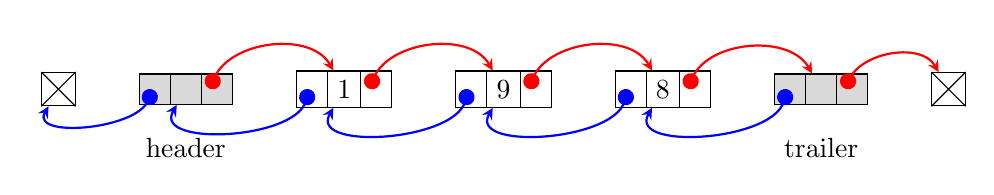
\begin{tikzpicture}[list/.style={rectangle split, rectangle split parts=3,
        draw, rectangle split horizontal}, >=stealth, start chain, node distance=.8cm]

        \node[on chain,draw,inner sep=6pt] (AA) {};
        \draw (AA.north east) -- (AA.south west);
        \draw (AA.north west) -- (AA.south east);

        \node[list, on chain, fill=gray!30] (header) {};
      \node[list,on chain] (A) {\nodepart{second}1};
      \node[list,on chain] (B) {\nodepart{second}9};
      \node[list,on chain] (C) {\nodepart{second}8};
      \node[list, on chain, fill=gray!30] (trailer) {};
      \node[on chain,draw,inner sep=6pt] (D) {};
      \draw (D.north east) -- (D.south west);
      \draw (D.north west) -- (D.south east);

      \draw[*->, red, thick] let \p1 = (header.three), \p2 = (header.center) in (\x1,\y2) to[out=80,in=120] (A);
      \draw[*->, red, thick] let \p1 = (A.three), \p2 = (A.center) in (\x1,\y2) to[out=80,in=120] (B);
      \draw[*->, blue, thick] let \p1 = (A.one), \p2 = (A.center) in (\x1,\y2) to[out=-80,in=-120] (header);
      \draw[*->, blue, thick] let \p1 = (header.one), \p2 = (header.center) in (\x1,\y2) to[out=-80,in=-120] (AA);

      \draw[*->, red, thick] let \p1 = (B.three), \p2 = (B.center) in (\x1,\y2) to[out=80,in=120] (C);
      \draw[*->, blue, thick] let \p1 = (B.one), \p2 = (B.center) in (\x1,\y2) to[out=-80,in=-120] (A);

      \draw[*->, red, thick] let \p1 = (C.three), \p2 = (C.center) in (\x1,\y2) to[out=80,in=120] (trailer);
      \draw[*->, blue, thick] let \p1 = (C.one), \p2 = (C.center) in (\x1,\y2) to[out=-80,in=-120] (B);
     \draw[*->, red, thick] let \p1 = (trailer.three), \p2 = (trailer.center) in (\x1,\y2) to[out=80,in=120] (D);
      \draw[*->, blue, thick] let \p1 = (trailer.one), \p2 = (trailer.center) in (\x1,\y2) to[out=-80,in=-120] (C);

      \node[below=of header, yshift=.5cm]{\alert{header}};
      \node[below=of trailer, yshift=.5cm]{\alert{trailer}};
    \end{tikzpicture}

{\large \faIcon{code}} How to add an element at the end of a list?
    \pause

        \scalebox{.85}{  
        \begin{algorithm}[H]
        \caption{addLast(header, trailer, element)}
        $x\gets trailer.prev$ \\
        $node \gets Node(element, x, trailer)$ \\
        $trailer.prev \gets node$ \\
        $x.next\gets node$
        \end{algorithm}
    }  
\end{frame}

\begin{frame}
    \frametitle{1.4 addBetween()}

To add an element between two nodes.

\begin{columns}
    \column{.4\textwidth}<1->
        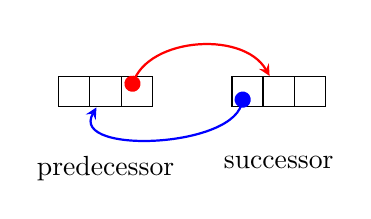
\begin{tikzpicture}[list/.style={rectangle split, rectangle split parts=3,
        draw, rectangle split horizontal}, >=stealth, start chain,]


      \node[list,on chain] (A) {};
      \node[list,on chain] (B) {};

      \draw[*->, red, thick] let \p1 = (A.three), \p2 = (A.center) in (\x1,\y2) to[out=80,in=120] (B);

      \draw[*->, blue, thick] let \p1 = (B.one), \p2 = (B.center) in (\x1,\y2) to[out=-80,in=-120] (A);


      \node[below=of A, yshift=.5cm]{\alert{predecessor}};
      \node[below=of B, yshift=.5cm]{\alert{successor}};
    \end{tikzpicture}
    \column{.6\textwidth}<2->
    {\large \faIcon{question-circle}} How to implement \texttt{addFirst()} and \texttt{addLast()} based on \texttt{addBetween()}?
\end{columns}


    \scalebox{.85}{  
        \begin{algorithm}[H]
            \caption{addBetween}
            $node\gets Node(element, predecessor, successor)$ \\
            $predecessor.next\gets node$ \\
            $successor.prev\gets node$
            \end{algorithm}
    }

\end{frame}

\begin{frame}
    \frametitle{1.5 Time Complexity}
    \begin{table}
        \caption*{Doubly Linked Lists}
        \begin{tabular}{ll}
          \toprule
          Operation & Time Complexity \\
          \midrule
          \texttt{addFirst()} & $O(1)$\\
          \texttt{addLast()} & $O(1)$ \\
          \texttt{removeFirst()} & $O(1)$ \\
          \texttt{removeLast()} & $O(1)$ \\
          \bottomrule
        \end{tabular}
    \end{table}    

\end{frame}

\begin{frame}
    \section{\textcolor{darkmidnightblue}{2. Array vs. Linked List}}
    There is not a one-size-fits-all solution.

\end{frame}

\begin{frame}
    \begin{table}
        \caption*{Array vs. Linked List}
        \begin{tabular}{ll}
          \toprule
          Array & Linked List \\
          \midrule
          Contiguous memory layout & Non-contiguous \\
          Fixed in size & Dynamic \\
          Allocated in compile time & Allocated at run time \\
          Use less memory & Use more memory \\
          Faster indexing  & Slower traversing \\
          Slower insertion and deletion & Faster insertion and deletion \\
          \bottomrule
        \end{tabular}
    \end{table} 
\end{frame}

\begin{frame}
    \frametitle{A General Tip in Java}

    \begin{tikzpicture}
        \node[fill=blue!30,blur shadow={shadow xshift=-0.5ex},
        text width=26em,anchor=south west,rounded corners]
        {\faIcon{lightbulb} \texttt{ArrayList} with \texttt{ArrayDeque} are preferable in many more use-cases than \texttt{LinkedList}. If you're not sure — just start with \texttt{ArrayList}.};
    \end{tikzpicture}

    \pause
    
\includegraphics[width=.85\textwidth]{week6/linked}

\end{frame}

\begin{frame}
    \section{\textcolor{darkmidnightblue}{3. Case Study}}
    It is adapted from \href{http://cslibrary.stanford.edu/105/LinkedListProblems.pdf}{18 linked list problems}.
\end{frame}

{\setbeamercolor{palette primary}{fg=black, bg=yellow}
\begin{frame}[standout]
  There are several different representations of a singly/doubly linked list:
  \begin{itemize}
    \item head
    \item head + tail
    \item header + trailer
  \end{itemize}
\end{frame}
}

\begin{frame}
    \frametitle{3.1 count()}
Given a \alert{\texttt{head}} of a singly linked list, return the count of a target element \texttt{k}.    

\pause
\scalebox{.85}{  
    \begin{algorithm}[H]
        \setstretch{1}
        \caption{count(head, k)}
        $cnt\gets 0$ \\
        $x\gets head$ \\
        \While{x $\neq$ null} {
            \If{x.item == k} {
                $cnt\gets cnt + 1$
            }
            $x\gets x.next$
        }
        \Return{cnt}
        \end{algorithm}
}
\end{frame}

\begin{frame}
    \frametitle{3.2 sortedInsert()}

    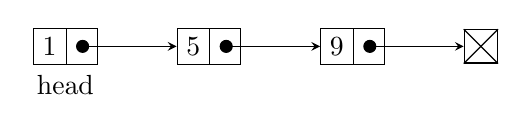
\begin{tikzpicture}[list/.style={rectangle split, rectangle split parts=2,
        draw, rectangle split horizontal}, >=stealth, start chain]
    
      \node[list,on chain] (A) {1};
      \node[list,on chain] (B) {5};
      \node[list,on chain] (C) {9};
      \node[on chain,draw,inner sep=6pt] (D) {};
      \draw (D.north east) -- (D.south west);
      \draw (D.north west) -- (D.south east);
      \draw[*->] let \p1 = (A.two), \p2 = (A.center) in (\x1,\y2) -- (B);
      \draw[*->] let \p1 = (B.two), \p2 = (B.center) in (\x1,\y2) -- (C);
      \draw[*->] let \p1 = (C.two), \p2 = (C.center) in (\x1,\y2) -- (D);

      \node[below=of A, yshift=1cm]{\alert{head}};
    \end{tikzpicture}

    To insert a node whose item is \texttt{k} so that the list is in ascending order.

    \pause
    \begin{itemize}
        \item \textbf{Case 1}: the list is empty.
        \item \textbf{Case 2}: the item of \texttt{head} is greater than or equal to \texttt{k}.
        \item \textbf{Case 3}: the item of \texttt{head} is less than \texttt{k}.
    \end{itemize}

\end{frame}

\begin{frame}

    \scalebox{.85}{  
        \begin{algorithm}[H]
            \setstretch{1}
            \caption{sortedInsert(head, k)}
            $node\gets Node(k)$ \\
            \If{head == null or head.item $\geq$ k} {
                \tcp{case 1 and case 2}
                $node.next\gets head$ \\
                $head\gets node$
            }\Else {
                \tcp{case 3}
                $x\gets head$ \\
                \While{x.next $\neq$ null and x.next.item $<$ k} {
                    $x\gets x.next$
                }
                $node.next\gets x.next$ \\
                $x.next\gets node$
            }
            \end{algorithm}
    }
\end{frame}

\begin{frame}
    \frametitle{3.3 reverseList()}
    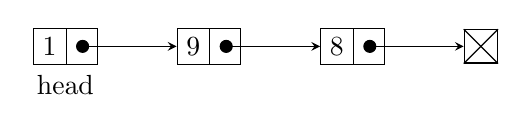
\begin{tikzpicture}[list/.style={rectangle split, rectangle split parts=2,
        draw, rectangle split horizontal}, >=stealth, start chain]
    
      \node[list,on chain] (A) {1};
      \node[list,on chain] (B) {9};
      \node[list,on chain] (C) {8};
      \node[on chain,draw,inner sep=6pt] (D) {};
      \draw (D.north east) -- (D.south west);
      \draw (D.north west) -- (D.south east);
      \draw[*->] let \p1 = (A.two), \p2 = (A.center) in (\x1,\y2) -- (B);
      \draw[*->] let \p1 = (B.two), \p2 = (B.center) in (\x1,\y2) -- (C);
      \draw[*->] let \p1 = (C.two), \p2 = (C.center) in (\x1,\y2) -- (D);

      \node[below=of A, yshift=1cm]{\alert{head}};
    \end{tikzpicture}

To reverse a list, and return the reversed \texttt{head}.

\begin{itemize}
    \item \textbf{Case 1}: the list is empty.
    \item \textbf{Case 2}: the size is 1.
    \item \textbf{Case 3}: the size is greater than 1.
\end{itemize}

\end{frame}

\begin{frame}[fragile]
\textbf{Two-pointers}

    \begin{columns}
        \column{.34\textwidth}
        \begin{verbatim}
next = cur.next
cur.next = pre
pre = cur
cur = next
        \end{verbatim}
        \column{.64\textwidth}
        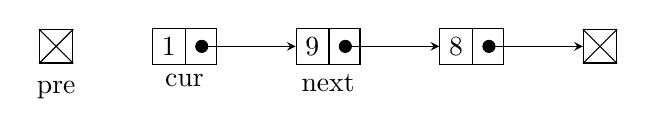
\begin{tikzpicture}[list/.style={rectangle split, rectangle split parts=2,
            draw, rectangle split horizontal}, >=stealth, start chain]
    
          \node[on chain, draw, inner sep=6pt] (prev) {};
          \draw (prev.north east) -- (prev.south west);
          \draw (prev.north west) -- (prev.south east);
          \node[list,on chain] (A) {1};
          \node[list,on chain] (B) {9};
          \node[list,on chain] (C) {8};
          \node[on chain,draw,inner sep=6pt] (D) {};
          \draw (D.north east) -- (D.south west);
          \draw (D.north west) -- (D.south east);
          \draw[*->] let \p1 = (A.two), \p2 = (A.center) in (\x1,\y2) -- (B);
          \draw[*->] let \p1 = (B.two), \p2 = (B.center) in (\x1,\y2) -- (C);
          \draw[*->] let \p1 = (C.two), \p2 = (C.center) in (\x1,\y2) -- (D);
    
          \node[below=of A, yshift=1cm]{\alert{cur}};
          \node[below=of prev, yshift=.9cm]{\alert{pre}};
          \node[below=of B, yshift=1cm]{\alert{next}};
        \end{tikzpicture}
\pause
        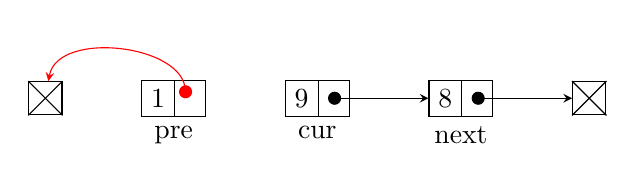
\begin{tikzpicture}[list/.style={rectangle split, rectangle split parts=2,
            draw, rectangle split horizontal}, >=stealth, start chain]
            \node[on chain, draw, inner sep=6pt] (null) {};
            \draw (null.north east) -- (null.south west);
            \draw (null.north west) -- (null.south east);
    
          \node[list,on chain] (A) {1};
          \node[list,on chain] (B) {9};
          \node[list,on chain] (C) {8};
          \node[on chain,draw,inner sep=6pt] (D) {};
          \draw (D.north east) -- (D.south west);
          \draw (D.north west) -- (D.south east);
          \draw[*->, red] let \p1 = (A.two), \p2 = (A.center) in (\x1,\y2) to[out=80,in=80] (null);
          \draw[*->] let \p1 = (B.two), \p2 = (B.center) in (\x1,\y2) -- (C);
          \draw[*->] let \p1 = (C.two), \p2 = (C.center) in (\x1,\y2) -- (D);
    
          \node[below=of A, yshift=1cm]{\alert{pre}};
          \node[below=of B, yshift=1cm]{\alert{cur}};
          \node[below=of C, yshift=1cm]{\alert{next}};
        \end{tikzpicture}
    \pause
        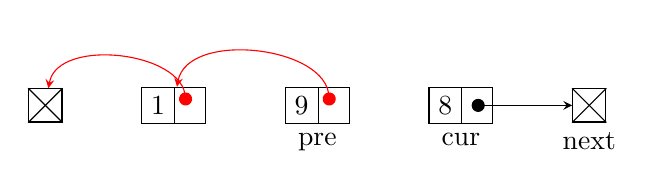
\begin{tikzpicture}[list/.style={rectangle split, rectangle split parts=2,
            draw, rectangle split horizontal}, >=stealth, start chain]
            \node[on chain, draw, inner sep=6pt] (null) {};
            \draw (null.north east) -- (null.south west);
            \draw (null.north west) -- (null.south east);
    
          \node[list,on chain] (A) {1};
          \node[list,on chain] (B) {9};
          \node[list,on chain] (C) {8};
          \node[on chain,draw,inner sep=6pt] (D) {};
          \draw (D.north east) -- (D.south west);
          \draw (D.north west) -- (D.south east);
          \draw[*->, red] let \p1 = (A.two), \p2 = (A.center) in (\x1,\y2) to[out=80,in=80] (null);
          \draw[*->, red] let \p1 = (B.two), \p2 = (B.center) in (\x1,\y2) to[out=80,in=80] (A);
          \draw[*->] let \p1 = (C.two), \p2 = (C.center) in (\x1,\y2) -- (D);
    
          \node[below=of B, yshift=1cm]{\alert{pre}};
          \node[below=of C, yshift=1cm]{\alert{cur}};
          \node[below=of D, yshift=1cm]{\alert{next}};
        \end{tikzpicture}
        \pause
        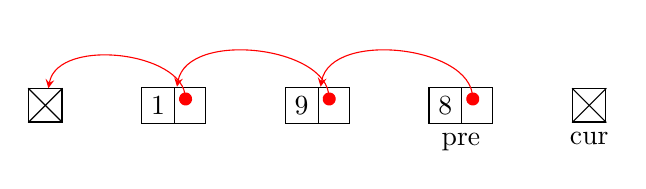
\begin{tikzpicture}[list/.style={rectangle split, rectangle split parts=2,
            draw, rectangle split horizontal}, >=stealth, start chain]
            \node[on chain, draw, inner sep=6pt] (null) {};
            \draw (null.north east) -- (null.south west);
            \draw (null.north west) -- (null.south east);
    
          \node[list,on chain] (A) {1};
          \node[list,on chain] (B) {9};
          \node[list,on chain] (C) {8};
          \node[on chain,draw,inner sep=6pt] (D) {};
          \draw (D.north east) -- (D.south west);
          \draw (D.north west) -- (D.south east);
          \draw[*->, red] let \p1 = (A.two), \p2 = (A.center) in (\x1,\y2) to[out=80,in=80] (null);
          \draw[*->, red] let \p1 = (B.two), \p2 = (B.center) in (\x1,\y2) to[out=80,in=80] (A);
          \draw[*->, red] let \p1 = (C.two), \p2 = (C.center) in (\x1,\y2) to[out=80,in=80] (B);
    
          \node[below=of C, yshift=1cm]{\alert{pre}};
          \node[below=of D, yshift=1cm]{\alert{cur}};
        \end{tikzpicture}
    \end{columns}

\end{frame}

\begin{frame}[fragile]
\begin{columns}
    \column{.4\textwidth}
    \begin{verbatim}
pre = null
cur = head
while (cur != null) {
    next = cur.next
    cur.next = pre
    pre = cur
    cur = next
}
return pre  
    \end{verbatim}
    \column{.64\textwidth}
    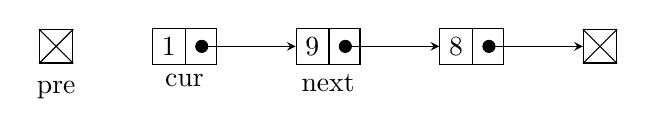
\begin{tikzpicture}[list/.style={rectangle split, rectangle split parts=2,
        draw, rectangle split horizontal}, >=stealth, start chain]

      \node[on chain, draw, inner sep=6pt] (prev) {};
      \draw (prev.north east) -- (prev.south west);
      \draw (prev.north west) -- (prev.south east);
      \node[list,on chain] (A) {1};
      \node[list,on chain] (B) {9};
      \node[list,on chain] (C) {8};
      \node[on chain,draw,inner sep=6pt] (D) {};
      \draw (D.north east) -- (D.south west);
      \draw (D.north west) -- (D.south east);
      \draw[*->] let \p1 = (A.two), \p2 = (A.center) in (\x1,\y2) -- (B);
      \draw[*->] let \p1 = (B.two), \p2 = (B.center) in (\x1,\y2) -- (C);
      \draw[*->] let \p1 = (C.two), \p2 = (C.center) in (\x1,\y2) -- (D);

      \node[below=of A, yshift=1cm]{\alert{cur}};
      \node[below=of prev, yshift=.9cm]{\alert{pre}};
      \node[below=of B, yshift=1cm]{\alert{next}};
    \end{tikzpicture}

    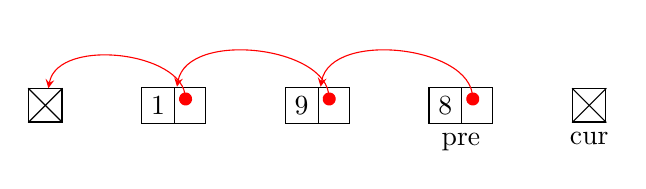
\begin{tikzpicture}[list/.style={rectangle split, rectangle split parts=2,
        draw, rectangle split horizontal}, >=stealth, start chain]
        \node[on chain, draw, inner sep=6pt] (null) {};
        \draw (null.north east) -- (null.south west);
        \draw (null.north west) -- (null.south east);

      \node[list,on chain] (A) {1};
      \node[list,on chain] (B) {9};
      \node[list,on chain] (C) {8};
      \node[on chain,draw,inner sep=6pt] (D) {};
      \draw (D.north east) -- (D.south west);
      \draw (D.north west) -- (D.south east);
      \draw[*->, red] let \p1 = (A.two), \p2 = (A.center) in (\x1,\y2) to[out=80,in=80] (null);
      \draw[*->, red] let \p1 = (B.two), \p2 = (B.center) in (\x1,\y2) to[out=80,in=80] (A);
      \draw[*->, red] let \p1 = (C.two), \p2 = (C.center) in (\x1,\y2) to[out=80,in=80] (B);

      \node[below=of C, yshift=1cm]{\alert{pre}};
      \node[below=of D, yshift=1cm]{\alert{cur}};
    \end{tikzpicture}

    {\large \faIcon{question-circle}} When to terminate the traversal?

    \pause
    {\large \faIcon{question-circle}} Can the code handle case 1 and 2?
\end{columns}

\end{frame}

\begin{frame}
    \scalebox{.85}{  
        \begin{algorithm}[H]
            \caption{reverseList(head)}
            $pre\gets null$ \\
            $cur\gets head$ \\
            \While{cur $\neq$ null} {
                $next\gets cur.next$ \\
                $cur.next\gets pre$ \\
                $pre\gets cur$ \\
                $cur\gets next$
            }
            \Return{pre}
            \end{algorithm}
    }

    {\large \faIcon{code}} Try to solve \href{https://leetcode.com/problems/reverse-linked-list/}{LeetCode: 206. Reverse Linked List} using Java or Python.

\end{frame}

\begin{frame}

    \section{\textcolor{darkmidnightblue}{Conclusion}} 
    \begin{enumerate}
        \item Doubly Linked List
        \item Array vs. Linked List
        \item Pointer moving
    \end{enumerate}
\end{frame}

\begin{frame}
    \frametitle{Course Preview}
{\large \faIcon{exclamation-triangle}} The next week's lesson will be held in Lab, and you will be asked to finish several programming assignments in class.

\end{frame}

\end{document}